In this section, we will demonstrate our brain-inspired simulation platform in terms of efficiency and scalability. Efficiency refers to how much speed up our platform can bring, compared to serial execution. Scalability refers to whether execution efficiency can increase as the number of available computing unit increases. 
As an example, we use the Lenet-5, a 7-layer convolutional neural network for handwritten digit recognition to test the performance of our brain-inspired simulation platform. Lenet-5 was proposed by Yann LeCun et al [6] and considered as the most classic convolutional neural network, which can achieve more than 98\% recognition accuracy on the MINST dataset. Its importance of brain-inspired calculation is self-evident. We believe that if we can implement Lenet-5 in our platform and achieve high speed than the existing technology, it will be sufficient to prove the feasibility and superiority of brain-inspired computation simulation based on data flow.
In contrast, we choose OpenMP, a pervasively used coarse-grained multi-threaded parallel computing model, to implement Lenet-5. The parameters of OpenMP have been carefully tuned to achieve the best performance

\subsection{Testbed}
The CPU of our testbed is dual sockets Intel(R) Xeon(R) CPU E5-2670 @ 2.60GH. Each sockets consists of 8 cores (16 threads). Each core has 32KB L1 cache and 256KB L2 cache. Each socket shares 20MB L3 cache. Testbed uses CentOS Linux system. All the source code is compiled on GCC4.6.2.
\subsection{Results}
 
%\textcolor{red}{Figure 10}
\begin{figure}[h]
\caption{Figure 10}
\centering
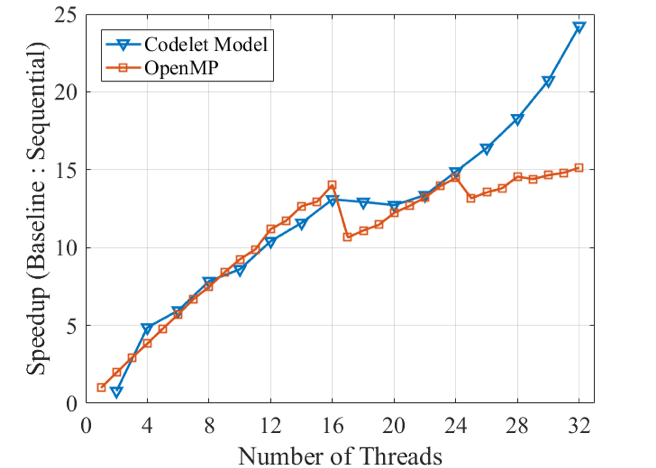
\includegraphics[width=1\textwidth]{Fig/figure10.png}
\end{figure}
Figure 10 shows the performance of two different implementation of Lenet-5 (Codelet model, OpenMP model). We manually change the number of thread and record the speed up against the sequential execution baseline. 
We can observe that when the number of threads available is less than 16, the speed up of both methods are comparable. However, when the number of threads increase over 16, the speed up of OpenMP shows a significant decrease. The reason lies in the dual-socket CPU employed by the testbed. Each socket has 16 threads, and no cache is shared between the sockets. When the computation work is allocated across the two sockets, all related data need to be read from the memory twice and synchronization operations will flush the cache twice, which will slow down the program. Our platform, on the other hand, is little effected by this situation. There are two main reasons: First, each TP stores the local data that are required by Codelets. These data need only be read into the cache once, saving memory access time; Second, the Codelet Abstract Machine Model ensures that the codelets within a TP can only run in the same cluster. Since the cluster is divided according to the processor hardware structure, which guarantees that Codelets from the same TP share the same L3 cache, there will be far less cache miss during execution.
When the number of available threads reaches more than 24, the execution efficiency of Codelet model begins to exceed that of OpenMP. When the number of threads reaches 32, the Codelet model provides 60% higher speed up than OpenMP, which shows that our platform has better scalability than OpenMP on multi-core and even many-core computing system.
We also examine the performance of our system against Tensrflow. The result is shown in Figure 11. The maximum speed up achieves 52.9%. We can conclude that, similar to the result against OpenMP, our platform demonstrates higher efficiency and scalability than Tensorflow. 
 
\textcolor{red}{Figure 11}
\begin{figure}[h]
\caption{Figure 11}
\centering
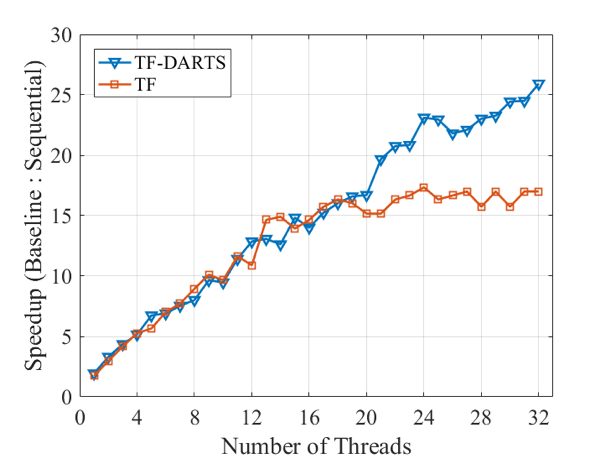
\includegraphics[width=1\textwidth]{Fig/figure11.png}
\end{figure}
In general, our platform, either alone or in combination with Tensorflow, shows higher efficiency and better scalability. Due to the fact that development of processor in the future is bound to increase core number, Codelet-based parallel brain-inspired computing simulation platform will have broader application prospects than traditional parallel acceleration model such as OpenMP.
